\documentclass[11pt,a4paper]{article}
\usepackage{amsmath,amssymb,amsthm,graphicx,hyperref,booktabs}
\usepackage[margin=2.5cm]{geometry}
\newtheorem{theorem}{Theorem}
\newtheorem{proposition}[theorem]{Proposition}
\newtheorem{lemma}[theorem]{Lemma}
\newtheorem{conjecture}[theorem]{Conjecture}
\theoremstyle{remark}\newtheorem{remark}[theorem]{Remark}
\newcommand{\ein}{\varepsilon_{\rm in}}
\newcommand{\eout}{\varepsilon_{\rm out}}
\newcommand{\fin}{f_{\rm in}}
\newcommand{\fout}{f_{\rm out}}
\graphicspath{{../FIGURES/}}

\title{Universe creation by tunnelling from laboratory data:\\
no manifold instanton, a unique canonical exponent, and a Smarr identity}
\author{Project Baby Universe --- Genesis Branch}
\date{21 October 2026 (Stage One manuscript, draft); addendum 22 October 2026}

\begin{document}
\maketitle

\begin{abstract}
We revisit the thin-wall model of a false-vacuum bubble (de Sitter interior, Schwarzschild exterior) and the
proposal of Farhi, Guth and Guven that such a bubble, too small to inflate classically, may tunnel into an
inflating, causally disconnected daughter universe. (i) We prove that, for every transition starting from regular,
time-symmetric, asymptotically flat (``laboratory'') data, the Euclidean exterior interpolating region cannot be
embedded in Euclidean Schwarzschild. The pseudomanifold encountered by Farhi--Guth--Guven is therefore forced. The
obstruction is tied to a sign change of the exterior extrinsic curvature while the wall recedes from the Euclidean
horizon; an interior sign change does not obstruct embedding. (ii) In the reduced canonical theory with the asymptotic
clock, the branch of the Euclidean momentum is fixed by analyticity. The competing branch is a horizon monodromy, which
in Euclidean language is the half-turn slicing jump. (iii) At $M=0$ the exponent is
$B=S_E[\text{instanton}]+\frac1{4G}(\sum A_{\max}-\sum A_{\min})$ in closed form; it equals the Coleman--De Luccia
exponent of the false vacuum when the false vacuum is the larger cap. (iv) For $M>0$ the exponent obeys a first law
$d\tilde B=({\rm Vol}^{\rm in}_E/8\pi G)\,d\Lambda_{\rm in}+A^W_E\,d\sigma-\Delta t^W_E\,dM$ and a Smarr identity
$B=-\frac{\Lambda_{\rm in}}{8\pi G}{\rm Vol}^{\rm in}_E-\frac\sigma2A^W_E-\frac M2\Delta t^W_E+\frac{\mathcal A}{4G}$.
This is a covariant expression in which the pseudomanifold enters only through one boundary term. Numerically, over
laboratory transitions $B\ge0.56\,B(M\!\to\!0)$ for all parameters and $B\ge B_{\rm CdL}$ when $\chi\gtrsim1.2\kappa$; for GUT-scale
parameters and gram-scale bubbles $B\sim10^6$. All statements are verified symbolically and numerically with an
open-source code.
\end{abstract}

\section{Introduction}
A spherical region of false vacuum separated from true vacuum by a domain wall can have an inflating interior even
though, seen from outside, it is a black hole \cite{BGG}. Farhi and Guth showed that such a configuration cannot
arise classically from regular initial data when the null energy condition holds \cite{FG}. Farhi, Guth and Guven
(FGG) asked whether quantum tunnelling could do it \cite{FGG}. Their canonical calculation was hampered by the choice
of slicing, and their Euclidean interpolation was not a manifold but a ``pseudomanifold'' with a conjectured action.
Fischler, Morgan and Polchinski found agreement within a Hamiltonian treatment \cite{FMP}. Later Hamiltonian work
extended these transitions to all signs of the cosmological constant \cite{dealwis,cespedes}. Holographic arguments
suggest that smooth saddles do not produce inflating bubbles \cite{Freivogel,FuMarolf}.

This paper makes the FGG difficulties precise and fixes the branch of the exponent within the reduced canonical
theory (see the Addendum: a residual ambiguity survives in the single-flip class). Section~\ref{sec:setup} fixes the model and conventions. Section~\ref{sec:global} summarises the global
structure. Section~\ref{sec:obstruction} proves the embedding obstruction. Section~\ref{sec:canonical} fixes the
branch of the canonical exponent. Sections~\ref{sec:M0}--\ref{sec:smarr} give the closed form at $M=0$, the first law
and the Smarr identity. Section~\ref{sec:num} collects numerical results and Section~\ref{sec:disc} the limitations.

\section{Model and conventions}\label{sec:setup}
Signature $(-,+,+,+)$, $c=1$. Interior $\fin=1-\chi^2r^2$, exterior $\fout=1-2GM/r-\eta^2r^2$ (here mostly $\eta=0$), wall
$S_{ab}=-\sigma h_{ab}$, $\kappa=4\pi G\sigma$. With $n$ pointing from interior to exterior, $K_{ab}=e^\mu_ae^\nu_b\nabla_\mu n_\nu$,
$[X]=X_+-X_-$, the Israel conditions $[K_{ab}]-h_{ab}[K]=-8\pi GS_{ab}$ reduce to
\begin{equation}
A_{\rm in}-A_{\rm out}=\kappa R,\qquad A\equiv n^r=\varepsilon\sqrt{f+\dot R^2},
\end{equation}
with $K_{\theta\theta}=RA$ and $K^\tau{}_\tau=(\ddot R+\tfrac12f')/A$. Using the identity $A_{\rm in}^2-A_{\rm out}^2=\fin-\fout$,
\begin{equation}
A_{\rm in}=\frac{\fin-\fout+\kappa^2R^2}{2\kappa R},\quad A_{\rm out}=\frac{\fin-\fout-\kappa^2R^2}{2\kappa R},\quad
\dot R^2+V(R)=0,\quad V=\fout-A_{\rm out}^2 .
\end{equation}
\begin{lemma}\label{lem:J1}
For $\sigma>0$, $(R,\ein,\eout)$ solves the unsquared junction condition iff $\dot R^2+V=0$ and $\varepsilon={\rm sgn}A(R)$ on
each side. The only spurious solutions of the squared equation are those with $\sigma<0$.
\end{lemma}
With $R=(2GM/L^2)^{1/3}z$, $L^4=(\chi^2-\eta^2+\kappa^2)^2+4\kappa^2\eta^2$: $V=1-g(z)/E$, $g=z^2-2\gamma/z+z^{-4}$,
$\gamma=(\chi^2-\eta^2-\kappa^2)/L^2$, $E=4\kappa^2L^{-8/3}(2GM)^{-2/3}$, and for $\eta=0$, $\eout={\rm sgn}(1-z^3)$,
$\ein={\rm sgn}(1-\gamma z^3)$.

\section{Global structure}\label{sec:global}
For $M<M_{\rm cr}=4\kappa^3/(Gg_{\min}^{3/2}L^4)$ there are a bounded branch ($0\to R_1\to0$) and a bounce branch ($\infty\to R_2\to\infty$).
\begin{proposition}\label{prop:G1}
(i) $\eout(R_2)=-1$ always. (ii) $\eout(R_1)=+1$ iff $E>2-2\gamma$ (regime A). (iii) At $E=2-2\gamma$, $R_1=2GM$.
(iv) In regime A, the flip radius $R_f$ with $A_{\rm out}(R_f)=0$ satisfies $R_1<R_f<R_2$.
\end{proposition}
The causal region occupied by the wall is determined by $({\rm sgn}f,\varepsilon,{\rm sgn}\dot R)$. We implemented this
coordinate-free itinerary and verified it against explicit integration in Kruskal and global de Sitter
coordinates: all 15 branches of our atlas agree (Fig.~\ref{fig:penrose}). Every inflating branch ends in region III, is
invisible from region I, and has a past-singular exterior, in accordance with \cite{FG}. The time-symmetric slice at $R_2$
contains the Einstein--Rosen bridge, a minimal sphere. Hence every classical history through it is singular to the past
and to the future, and a transition to it must replace its past.

\begin{figure}[t]\centering
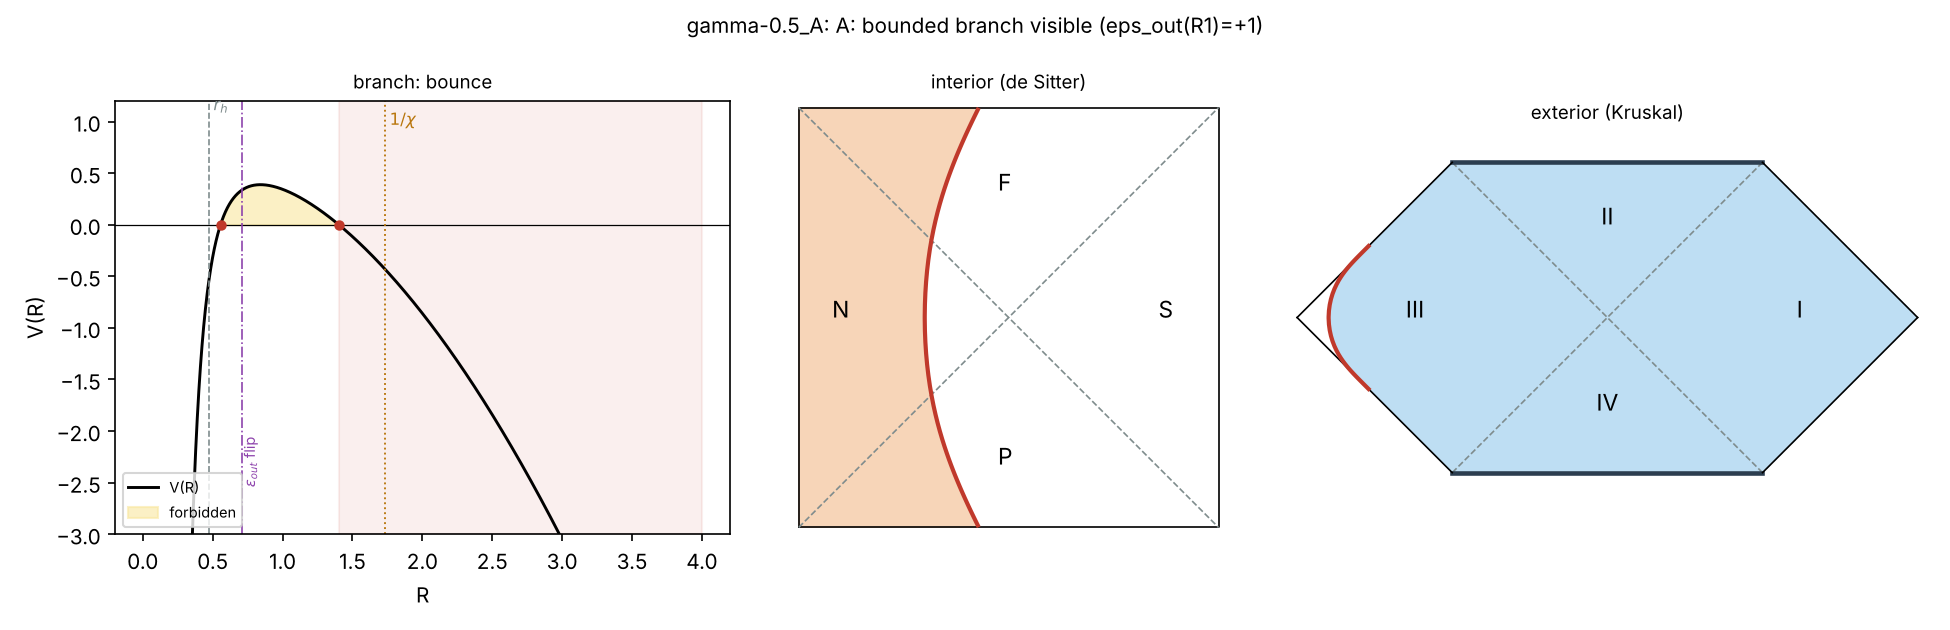
\includegraphics[width=\textwidth]{penrose_gamma-0.5_A_bounce.png}
\caption{Inflating bounce branch ($\gamma=-0.5$, regime A): effective potential, interior de Sitter diagram, exterior
Kruskal diagram, all drawn from integrated trajectories.}\label{fig:penrose}
\end{figure}

\section{The exterior embedding obstruction}\label{sec:obstruction}
Let $\mathcal C$ be the $(r,t_E)$ section of Euclidean Schwarzschild (a smooth cigar), with polar coordinates
$(\rho,\theta)$, $\theta=t_E/4GM$. The Euclidean wall obeys $R'^2=V$, $\fout\,dt_E/d\tau_E=A_{\rm out}(R)$.
\begin{theorem}[no manifold instanton]\label{thm:NG3}
Suppose that (H1) the half-bounce runs from $R_1$ to $R_2>R_1$ with $R'>0$; (H2) $A_{\rm out}$ has a single simple zero in
$(R_1,R_2)$ with $A_{\rm out}(R_1)>0>A_{\rm out}(R_2)$; (H3) the initial and final exterior slices are the totally geodesic slices
($\theta=0$ ray; broken line through the tip at angles $\theta_D,\theta_D+\pi$); (H4) the exterior region is an oriented surface
locally isometric to $\mathcal C$, with boundary initial slice $\cup$ wall $\cup$ final slice. Then the local isometry is not
injective.
\end{theorem}
\begin{proof}[Proof sketch]
Orientation places the region outside the $\varepsilon=+1$ arc, inside the $\varepsilon=-1$ arc, counterclockwise of the initial
ray, and clockwise of the final ray. If the map were injective, the multiplicity would be 1 on the region, 0 off it,
and would jump by one across each boundary piece. Monotonicity of $R$ puts the $\varepsilon=-1$ arc outside the $\varepsilon=+1$
arc. If either arc wraps by $\ge2\pi$, a radial segment between consecutive windings has multiplicities 0 and 1 at its
ends with no crossing between them. Otherwise, at infinity the multiplicity is 1 exactly on the counterclockwise arc
$(0,a)$, $a\equiv\theta_D+\pi$, while just outside the $\varepsilon=-1$ arc it is 0. A case analysis in $\theta_D$ produces in each case
an angle at which these two requirements conflict. The full proof is in the companion file \texttt{NO\_GO\_THEOREMS.md}.
\end{proof}
For the dS$|$Schwarzschild model, every regime-A transition satisfies (H1)--(H4). Degree-theory multiplicity maps confirm
the result: they take values outside $\{0,1\}$ (Fig.~\ref{fig:mult}), including negative values for small $M$, where the
wall winds dozens of times around the horizon. Regime-B transitions ($\eout=-1$ throughout) are also non-manifold
numerically, with $|\theta_D|>\pi$ over the whole regime. The interior is not obstructed: models with an $\ein$ flip have
embedded interiors, because there the wall approaches the Euclidean horizon.

\begin{figure}[t]\centering
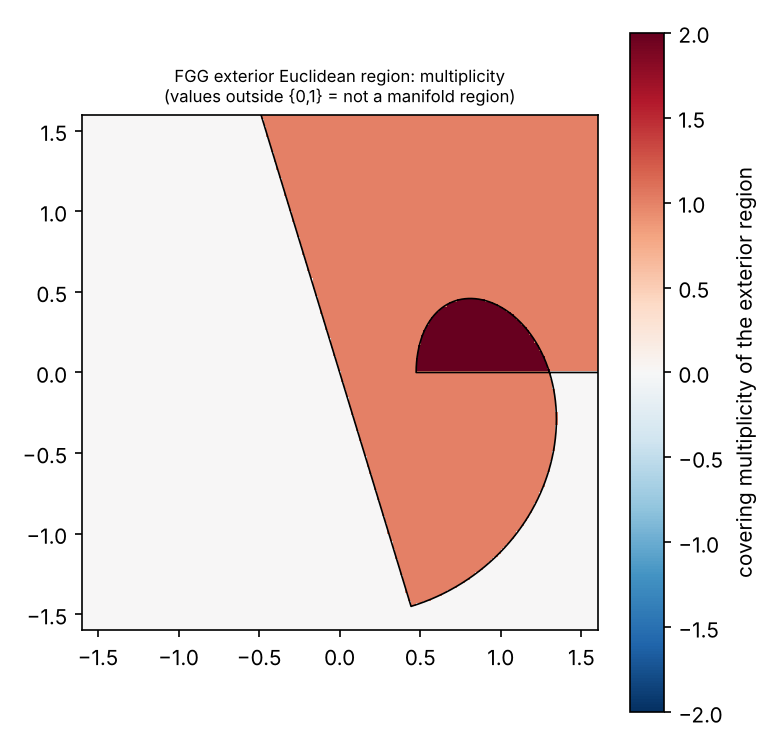
\includegraphics[width=0.45\textwidth]{pseudomanifold_multiplicity.png}
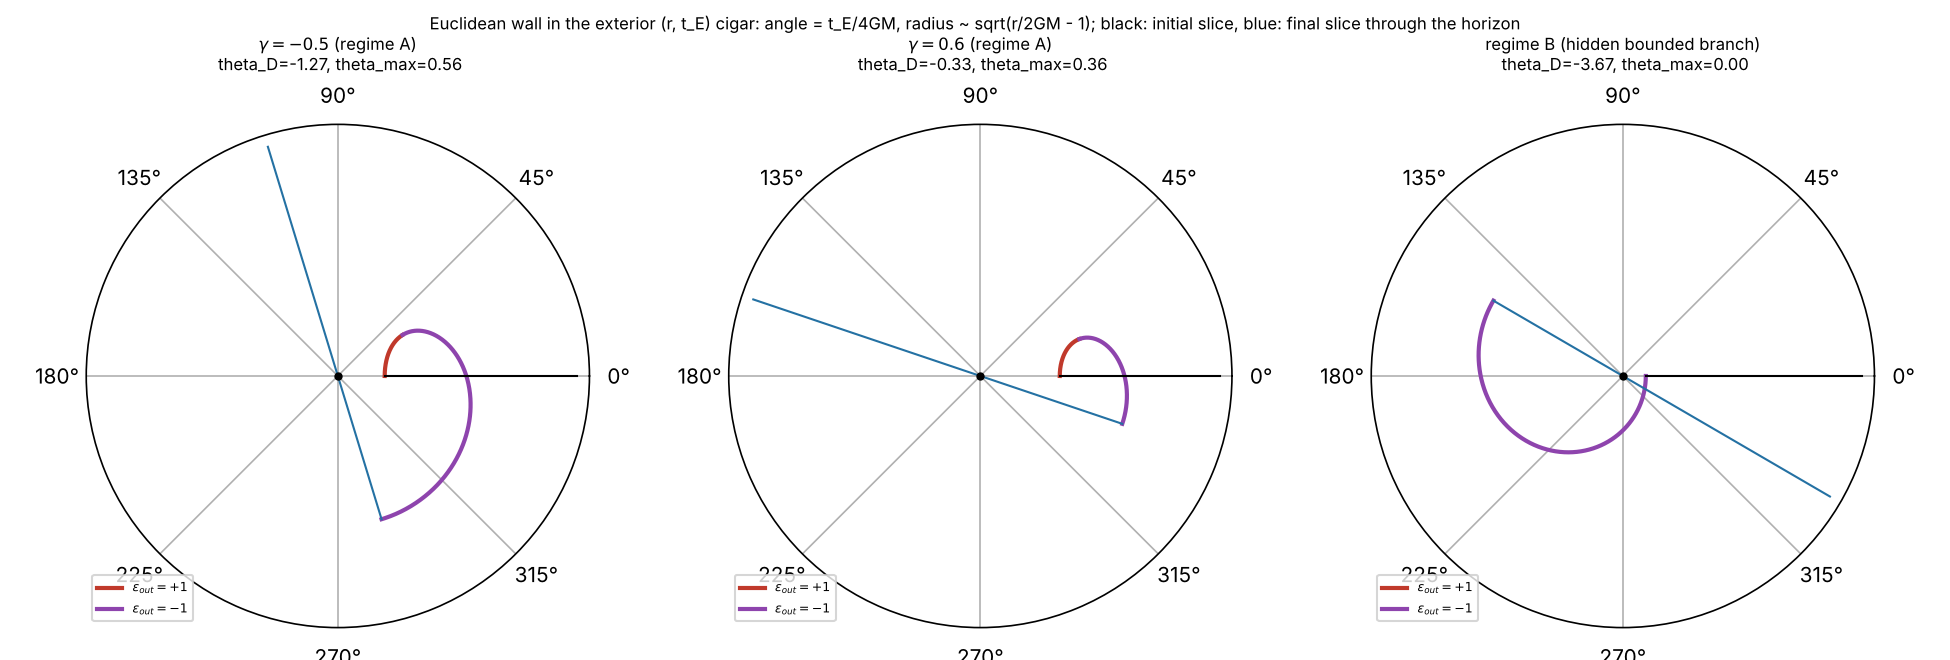
\includegraphics[width=0.53\textwidth]{euclidean_wall_exterior.png}
\caption{Left: covering multiplicity of the exterior Euclidean region for a regime-A transition. Right: the
Euclidean wall in the cigar for three models.}\label{fig:mult}
\end{figure}

\section{The canonical exponent and its branch}\label{sec:canonical}
With the asymptotic Killing time as clock and $H=M$, Hamilton's equation $\partial P/\partial M|_R=dt/dR$ gives
\begin{equation}
P=\frac RG\Big[\operatorname{artanh}\frac{\dot R}{A_{\rm out}}-\operatorname{artanh}\frac{\dot R}{A_{\rm in}}\Big],\qquad
2\sqrt{\fin\fout}\cosh\frac{GP}R=\ein\eout(\fin+\fout-\kappa^2R^2),
\end{equation}
together with $\partial P/\partial\Lambda_{\rm in}|_{R,M}=-\frac1{8\pi G}\frac{4\pi R^3}3\frac{dt_{\rm in}}{dR}$ and
$\partial P/\partial\sigma|_{R,M}=-4\pi R^2\frac{d\tau}{dR}$. Under the barrier $P=iP_E$,
$P_E=\frac RG(\Theta_{\rm out}-\Theta_{\rm in})$ with $(A,\sqrt V)=\sqrt f(\cos\Theta,\sin\Theta)$, and $B=2\int_{R_1}^{R_2}P_E\,dR$.
\begin{proposition}[branch selection]
On $(R_1,R_2)$ we have $f\ge V>0$ on both sides, so $P$ is analytic there. Its branch points are the turning points and
the horizons $f=0$; the flip radius is a regular point. The WKB phase is the analytic continuation along the barrier,
$\Theta={\rm atan2}(\sqrt V,A)\in[0,\pi]$. The principal branch differs by a horizon monodromy
($P\to P\pm i\pi R/G$, $t\to t\pm i\beta/2$), which is the Euclidean half-turn slicing jump of FGG. The principal branch gives
$B<0$ in 41 of 45 test models.
\end{proposition}

\section{Closed form at \texorpdfstring{$M=0$}{M=0}}\label{sec:M0}
\begin{theorem}\label{thm:M0}
Let $M=0$, $R_0=2\kappa/L^2$, $p=-A_{\rm out}(R_0)$, $q=A_{\rm in}(R_0)$ ($p+q=\kappa R_0>0$). Then
\begin{equation}
S_E=-\frac{\pi R_0^2}{2G}\Big[\frac1{1+p}+\frac1{1+q}\Big],\qquad
B=\frac{\pi R_0^2}{2G}\frac{p+q+2p_+q_+}{(1+|p|)(1+|q|)}=S_E+\frac1{4G}\Big(\sum A_{\max}-\sum A_{\min}\Big),
\end{equation}
the sums running over the extremal spheres of the instanton's time-symmetric slice. If $q<0$, then $B=B_{\rm CdL}$, the
decay exponent of the false vacuum.
\end{theorem}
The proof uses $J(s)=\int_0^1x\,{\rm atan2}(\sqrt{1-x^2},sx)dx=\pi/4(1+s)$ ($s\ge0$), $\pi/2-\pi/4(1-s)$ ($s<0$), together with
the cap volumes. Gravitational $O(4)$ bounces of a quartic scalar converge to $B_{\rm CdL}$ as $O(w)$ in the wall width
(0.18\% at $w=0.005$).

\section{First law and Smarr identity}\label{sec:smarr}
\begin{theorem}\label{thm:smarr}
Let $\tilde B=B-\mathcal A/4G$, where $\mathcal A$ collects the endpoint areas ($\pm4\pi R_i^2$ where the wall is an extremal sphere of
its slice, plus $4\pi/\chi^2$ if the final slice contains the de Sitter equator). Then, within a regime,
\begin{equation}
d\tilde B=\frac{{\rm Vol}^{\rm in}_E}{8\pi G}d\Lambda_{\rm in}+A^W_E\,d\sigma-\Delta t^W_E\,dM,\qquad
B=-\frac{\Lambda_{\rm in}}{8\pi G}{\rm Vol}^{\rm in}_E-\frac\sigma2A^W_E-\frac M2\Delta t^W_E+\frac{\mathcal A}{4G},
\end{equation}
where ${\rm Vol}^{\rm in}_E$ is the Euclidean interior 4-volume of the full bounce, $A^W_E$ the wall's Euclidean area, and
$\Delta t^W_E$ the exterior Euclidean Killing time along the wall.
\end{theorem}
\begin{proof}
The first law is the Euclidean continuation of the three Hamilton--Jacobi relations, with endpoint contributions
$2P_E(R_i)dR_i=d(\mathcal A/4G)$. The Smarr identity follows from Euler's relation for $\tilde B$, which is homogeneous of degree 2
under $(\Lambda,\sigma,M)\to(\lambda^{-2}\Lambda,\lambda^{-1}\sigma,\lambda M)$.
\end{proof}
The first two terms are the on-shell action of the interior region and the wall. The exterior pseudomanifold
contributes only $-\frac M2\Delta t^W_E$, which tends to zero as $M\to0$ even though the Euclidean winding diverges.
Integrating the first law in $M$ from the $M=0$ instanton gives $B(M)=S_E^{(0)}+\mathcal A(M)/4G-\int_0^M\Delta t^W_E\,dM'$.
Numerically the identity holds to $2.5\times10^{-8}$ over 45 models.

\section{Numerical results}\label{sec:num}
Over regime A (laboratory data) the ratio $B/B(M\to0)$ is bounded below by $0.56$ for all $\gamma\in[-0.95,0.95]$, and by $1$
for $\gamma\gtrsim0.2$, where $B(M\to0)=B_{\rm CdL}$ (Fig.~\ref{fig:B}). For GUT-like parameters,
$\sigma^{1/3}=\rho^{1/4}=10^{16}$\,GeV ($M_{\rm cr}\approx5.6$\,g), $B=133$ only for nanogram (sub-Planckian, see Addendum) masses, while $B\approx7\times10^4$ at
$10^{-3}M_{\rm cr}$ and $4\times10^6$ at $0.5M_{\rm cr}$.

\begin{figure}[t]\centering
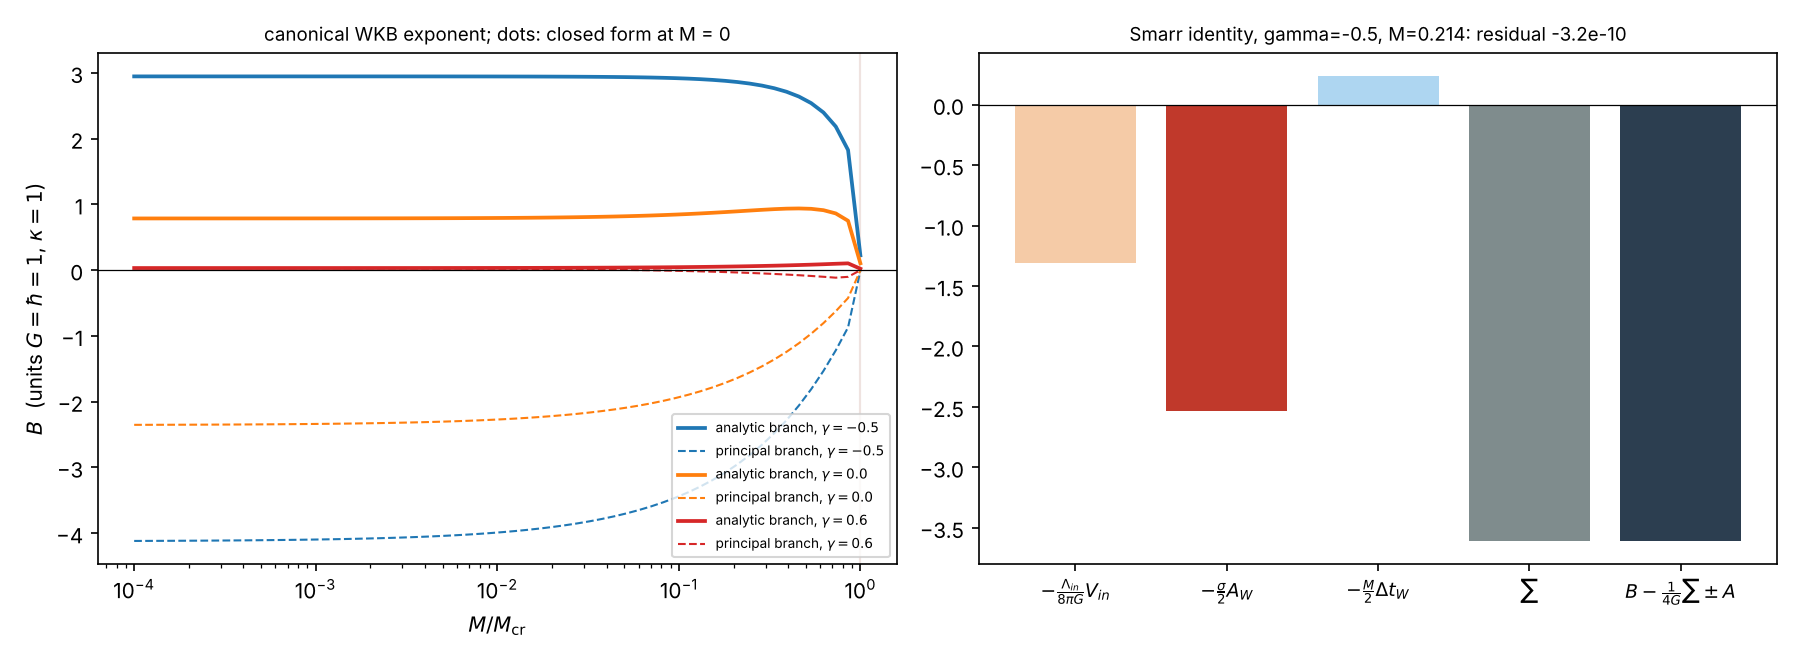
\includegraphics[width=\textwidth]{tunnelling_exponent.png}
\caption{Left: $B(M)$ for the analytic (solid) and principal (dashed) branches; dots: Theorem~\ref{thm:M0}. Right: the
terms of the Smarr identity.}\label{fig:B}
\end{figure}

\section{Discussion and limitations}\label{sec:disc}
The three obstructions to universe creation in an asymptotically flat parent, classical (Farhi--Guth), initial-data
(bag-of-gold minimal sphere) and semiclassical (Theorem~\ref{thm:NG3}), share one origin: the creation of a closed
marginally trapped surface in the exterior. Within the reduced canonical theory, the branch of the exponent is fixed and the exponent is covariantly
expressible; the remaining ambiguity is located in the Addendum. Open problems: the exact quantum amplitude (an exact solution is possible at
$M=0$, where the constraint becomes an ODE in the momentum representation); whether Lorentzian path integrals select the
same contour; prefactors; thick-wall versions of Theorems~\ref{thm:NG3} and \ref{thm:smarr}; non-spherical perturbations.
Our novelty claims are provisional pending comparison with the full texts of \cite{FGG,FMP,dealwis,cespedes}.


\section*{Addendum (22 October 2026): corrections and later results}
This manuscript reports Stage One only. Later work (Phases II--VI and the roadmap round; the documents named below are in the
accompanying repository) corrects or sharpens the following points.
\begin{enumerate}
\item \emph{The ambiguity is located, not removed} (PHASE\_III). Analyticity fixes the branch of $P$ (Proposition above), but every formulation
hides the FGG datum in one place: the boost-angle convention of a flipped normal, equivalently the relative normalisation of the orientation
sectors. Exactly one ambiguity survives: in the single-flip class two consistent exponents remain, $B_{\rm an}$ and
$B_{\rm sq}=\frac2G\int R\arccos|C|\,dR<B_{\rm an}$, with a universal Stokes multiplier $\sqrt2$. The multiplier is now confirmed by exact integration of the
momentum-space squared constraint at $M=0$.
\item \emph{Where the ambiguity lives} (ROADMAP Theorem S4). A laboratory transition is double-flip, hence unambiguous, iff $\kappa<\chi$ and
$M<M_{\rm sd}=(\chi^2-\kappa^2)/2G\chi^3$; the boundary is $R_2=1/\chi$. In the single-flip class, a sector-independent probability current gives
$2e^{-B_{\rm sq}}$, while $e^{-B_{\rm an}}$ requires an entropy-weighted daughter measure (ROADMAP Q9.3--Q9.4).
\item \emph{T5 status} (ROADMAP Part A). For light walls, T5 is a theorem with an explicit universal law
$B=B_{\rm CdL}\,\Phi\big((R_{\rm CdL}/R_M)^2\big)\ge4\pi^2\sigma^2R_M^2/\rho$. It implies the frontier
$B\ge\frac43\sqrt{\pi/2}\sqrt{B_{\rm CdL}(M/m_P)(R_M/\ell_P)}$, so in any semiclassically controlled regime $P\le10^{-23}$. Elsewhere $B\ge0.564\,B(0)$ remains
numerical.
\item \emph{Masses} (PHASE\_V). ``Picogram'' should read nanogram. These masses are below the Planck mass, so the black hole is not semiclassical. For
$M\gtrsim10m_P$ the GUT exponent is $B\gtrsim7\times10^4$.
\item \emph{The daughter needs no boundary condition, but the clock folds back} (ROADMAP Part D). The finite-time ``edge'' of the daughter channel is a
coordinate singularity of the static-frame momentum. Along every daughter $dt_\infty/d\tau<0$ (region III), so unitary boundary-clock evolution produces the
time-reversed daughter. The expanding daughter is a negative-flux (Klein-type) channel. This is consistent with the holographic and GSL obstructions
\cite{Freivogel,Wall}.
\item \emph{Literature.} The FMP abstract states that agreement with the Euclidean method requires degenerate metrics \cite{FMP}; Ansoldi and Tanaka resolve
slicing discrepancies with a smooth time slice \cite{AT}. Both are consistent with the results above. A full-text comparison is still pending.
\end{enumerate}

\begin{thebibliography}{99}
\bibitem{BGG} S.~K.~Blau, E.~I.~Guendelman, A.~H.~Guth, Phys.\ Rev.\ D \textbf{35}, 1747 (1987).
\bibitem{FG} E.~Farhi, A.~H.~Guth, Phys.\ Lett.\ B \textbf{183}, 149 (1987).
\bibitem{FGG} E.~Farhi, A.~H.~Guth, J.~Guven, Nucl.\ Phys.\ B \textbf{339}, 417 (1990).
\bibitem{FMP} W.~Fischler, D.~Morgan, J.~Polchinski, Phys.\ Rev.\ D \textbf{41}, 2638 (1990); \textbf{42}, 4042 (1990).
\bibitem{CdL} S.~Coleman, F.~De Luccia, Phys.\ Rev.\ D \textbf{21}, 3305 (1980).
\bibitem{Israel} W.~Israel, Nuovo Cim.\ B \textbf{44}, 1 (1966).
\bibitem{dealwis} S.~de Alwis, F.~Muia, V.~Pasquarella, F.~Quevedo, Fortschr.\ Phys.\ (2020), arXiv:1909.01975.
\bibitem{cespedes} S.~C\'espedes, S.~de Alwis, F.~Muia, F.~Quevedo, Phys.\ Rev.\ D \textbf{109}, 105027 (2024), arXiv:2307.13614.
\bibitem{Freivogel} B.~Freivogel, V.~Hubeny, A.~Maloney, R.~Myers, M.~Rangamani, S.~Shenker, JHEP \textbf{03} (2006) 007.
\bibitem{FuMarolf} Z.~Fu, D.~Marolf, JHEP \textbf{11} (2019) 040.
\bibitem{AJ} A.~Aguirre, M.~C.~Johnson, Phys.\ Rev.\ D \textbf{72}, 103525 (2005).
\bibitem{CHY} P.~Chen, Y.-C.~Hu, D.-h.~Yeom, Phys.\ Rev.\ D \textbf{94}, 024044 (2016).
\bibitem{UA} A.~Ulvestad, A.~Albrecht, Phys.\ Rev.\ D \textbf{85}, 103527 (2012).
\bibitem{Wall} A.~C.~Wall, Class.\ Quant.\ Grav.\ \textbf{30}, 165003 (2013).
\bibitem{Penrose} R.~Penrose, Phys.\ Rev.\ Lett.\ \textbf{14}, 57 (1965).
\bibitem{Parke} S.~Parke, Phys.\ Lett.\ B \textbf{121}, 313 (1983).
\bibitem{AT} S.~Ansoldi, T.~Tanaka, J.\ Exp.\ Theor.\ Phys.\ \textbf{120}, 460 (2015), arXiv:1410.6202.
\end{thebibliography}
\end{document}
